\subsection{Sprint End Organisation}

\begin{frame}{The First Sprint Review}
	This meeting had some fundamental problems:
	\begin{itemize}
		\item No feedback from the clients.
		\item Technical problems with the demonstrations.
		\item Obscure presentations.
	\end{itemize}
	\vspace{\baselineskip}
	So, a Sprint End specialist was appointed.
\end{frame}

\begin{frame}{Sprint End Collaboration}
	As the specialist was in this group, we had several tasks in connection with the sprint reviews:
	\begin{itemize}
		\item<1> Instructing the groups on how to present their progress.
		\item<2> Testing that all applications worked together.
		\item<3> Helping groups with last-minute integration problems.
		\item<4> Conduct the client install party.
		\item<5> Host the sprint review meeting.
	\end{itemize}
\end{frame}


\subsection{The Remote Database}

\begin{frame}{Enabling Syncronization}
	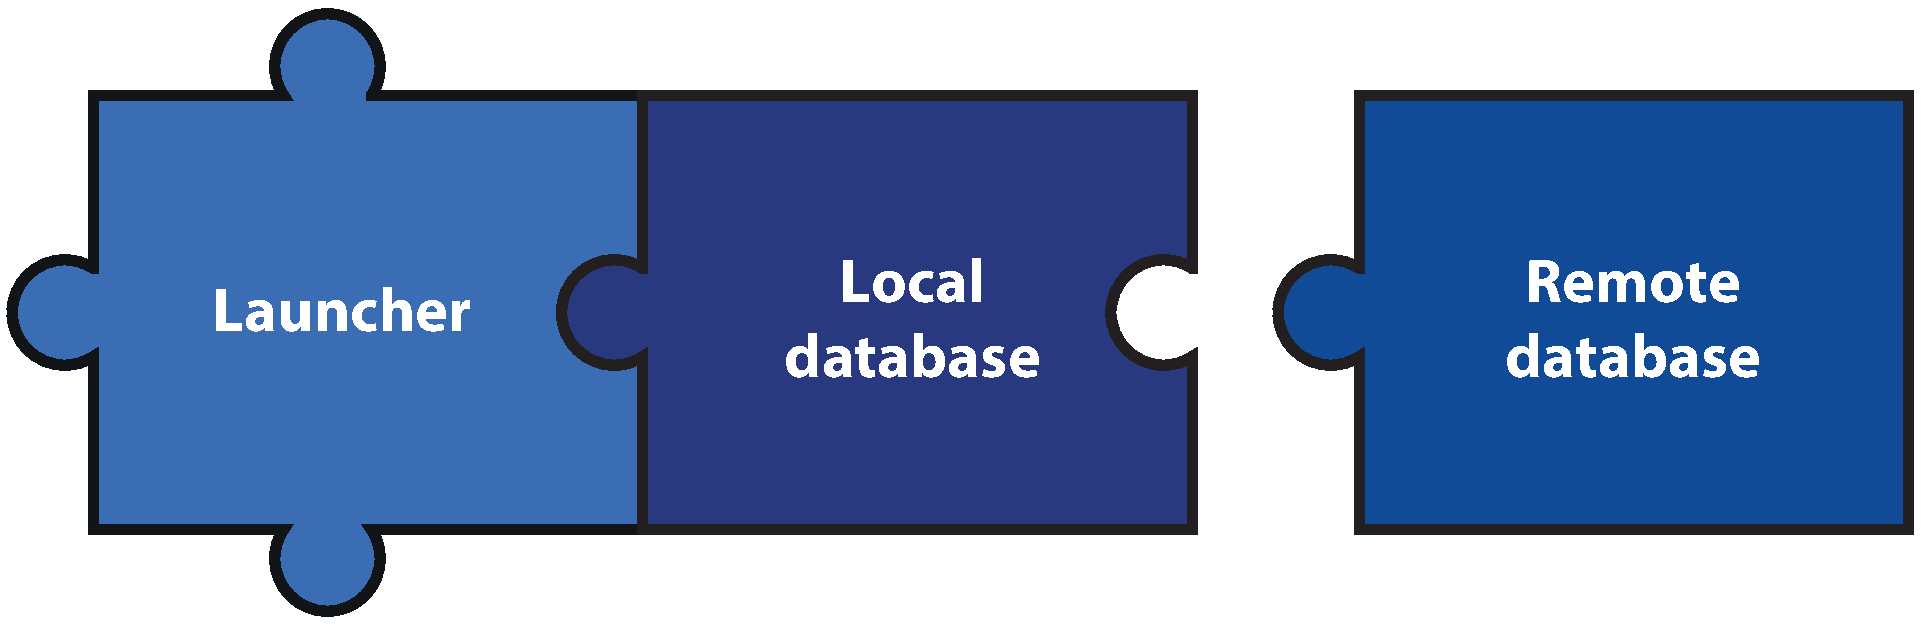
\includegraphics[height=3.5cm]{images/giraf-puzzle}
\end{frame}

\begin{frame}{Implementation Issues}
	The implementation this resulted in several problems:
	\begin{itemize}
		\item<1,4> Inconsistencies between the two databases.
		\item<2,4> Inconsistencies between the applications and the modified local database.
		\item<3,4> The inability of \textit{Pictosearch} to handle large numbers of pictograms.
	\end{itemize}
	\pause[4]
	\begin{block}{Frederic P. Brooks (1995)}
    	\textit{``All programmers are optimists.''}
   	\end{block}
\end{frame}


\subsection{Informal Collaboration}

\begin{frame}{Informal Collaboration}
	``Ad hoc'' collaboration was prevalent throughout the project:
	\begin{itemize}
		\item<1> Issues in inter-application communication.
		\begin{itemize}
			\item<1> The refactoring of OasisLib.
		\end{itemize}
		\item<2> Ideas from one group, that concerned other groups.
		\begin{itemize}
			\item<2> Our concept of an improved profile selector.
		\end{itemize}
	\end{itemize}
	\vspace{\baselineskip}
	\pause[3]
	This worked out well, due to a friendly ``open-door'' culture.
\end{frame}

